\documentclass[10pt]{article}

\usepackage{todonotes}
\usepackage{algorithm}
\usepackage{url}
\usepackage[margin=1in]{geometry}
\usepackage[noend]{algpseudocode}
\usepackage{mdframed}
\usepackage{amsmath}
\usepackage{amsthm}
\usepackage{paralist}
\usepackage{amsfonts}
%-----cut here with a sharp machete or an 19.95 ginsu knife
%************************************************************************
%* BNF.tex								*
%* 									*
%* plain tex macros for formatting grammars				*
%*									*
%* Erik Quanstrom 							*
%* 10. November 1990							*
%************************************************************************

%things to fix:
%	make configurable
%	work with texinfo

\gdef\actifygrammarchars{%
	\catcode`\>\active%
	\catcode`\<\active%
	\catcode`\:\active%
	\catcode`\"\active%
	\catcode`\;\active%
	\catcode`\.\active%
	\catcode`\|\active%
	\catcode`\,\active}

\gdef\deactifygrammarchars{%
	\catcode`\>12%
	\catcode`\<12%
	\catcode`\:12%
	\catcode`\;12%
	\catcode`\.12%
	\catcode`\|12%
	\catcode`\,12}

\newif\ifquote
\quotefalse

\begingroup
   \actifygrammarchars
   \gdef>{\/\endgroup$\rangle$\relax}
   \gdef<{$\langle$\begingroup\sl}
   \gdef:{$\rightarrow$}

   \begingroup
	\catcode`\"\active
	\gdef"{\ifquote%
		'\endgroup\quotefalse%
	   \else%
		\quotetrue\begingroup\deactifygrammarchars\bf`%
	\fi}%
   \endgroup

   \gdef;{\hfill\break}
   \gdef.{\relax}
   \gdef|{$\vert$}
   \gdef,{;\hbox to 1cm{\hfill}}
\endgroup

\def\begingrammar{%
	\begingroup
	\advance\leftskip by 1cm%
	\parindent=-1cm%
	\actifygrammarchars%
	\def\endgrammar{\endgroup}
	\parskip 1ex%
	\relax
}

%
%
%
\def\ul{\lower .2ex\hbox to 1ex{\hrulefill}\relax}%



\newtheorem{defn}{\textbf{Definition}}
\newtheorem{thm}{\textbf{Theorem}}
\newtheorem{cor}{\textbf{Corollary}}
\newtheorem{lemma}{\textbf{Lemma}}

% \newcommand{\AND}{{\sf AC$^{\mbox{{\small 3}}}$N}}
\newcommand{\sink}{{\sf CCNSink}}

\begin{document}

% ccn gateway and bridge
\title{CCNSink: Application-Layer Middleware for TCP/IP and Content Centric Network Interoperability}
\author{Christopher A. Wood \\ {\tt woodc1@uci.edu}}
\date{\today}

\maketitle
\begin{abstract}
With the growing presence of data streaming services and applications in today's Internet, content-centric networks (CCNs) are an increasingly attractive design alternative to the traditional IP-based host-oriented architecture. CCNs emphasize content by making it directly addressable and routable within the network, in contrast to addressable hosts and interfaces. This fundamental difference leads to vastly different mechanisms to publish and retrieve content and enable peer-to-peer communication. Named Data Networking (NDN) and its sibling implementation - CCNx - is one particular CCN design that has received considerable academic and industry attention. Despite the many promising benefits, there has been little research into the NDN deployment strategy. Clearly, incremental deployment is the only viable solution. During this integration phase, however, there will undoubtedly be a need for IP-based (NDN-based) hosts to communicate with and retrieve content from NDN-based (IP-based) hosts. To this end, we present  \sink, a middleware application to support interoperability between these different networking architectures with minimal application and transport layer modifications via semantic translation between the communication mechanisms used in both networks. We discuss the implementation details at length and study the performance overhead induced by this gateway and the message RTT is studied in various communication settings.
\end{abstract}

% \category{H.4}{TODO}{TODO}
% \category{D.2.8}{TODO}{TODO}[TODO]
% \terms{NDN/CCN; CCN Deployment; Network Gateway; Middleware}

%\keywords{TODO} % NOT required for Proceedings

\section{Introduction}
At its core, the design and architecture of today's Internet is communication-based packet switching network. Since its inception, it has been retrofitted with a variety of transport and application layer protocols and middleware to support a growing set of consumer applications, such as the Web, email, and perhaps most importantly in recent times, media streaming services. The latter type of applications are bandwidth-intensive content distribution applications which leverage the underlying communication-based network as a distribution network, leading to a massive consumption of vital networking resources. 

Information-centric networks (ICNs) are a new class of network architecture designs that aim to address this increasingly popular type of network traffic by decoupling data from its source and shifting the emphasis of addressable content from hosts and interfaces to content \cite{first}. By directly addressing content instead of hosts, content dissemination and security can be ``distributed'' throughout the network in the sense that consumers requests for content are satisifed by \emph{any} resource in the network (i.e., not necessarily the original producer). For example, routers close to consumers may cache content with a particular name and then satisfy all content requests that match the content's name. In-network caching and data-centric security measures are two of the defining characteristics of these new network designs. 

As of today there are several information-centric networking proposals being explored as alternative designs to today's Internet; Named Data Networking (NDN) \cite{NDNtech} is one of the more promising designs that is still an active area of active research (see \url{www.named-data.net} for more information). As a replacement for IP-based networks, the complete adoption of NDN, or any one of these designs, will realistically need to be done by slow and continual integration and replacement of IP-based networking resources with NDN-based resources. Currently, however, there is no engineering plan to support the IP-to-ICN integration without significant software modification and application, transport, or network layer source code modifications.

Consequently, the primary objective of this work is to aid the integration of future content-centric networking resources into the existing IP-centric Internet by providing an application and transport layer gateway between IP and NDN resources. Application-layer traffic corresponding to protocols such as HTTP, FTP, SMTP, IMAP, etc. will be translated by middleware running in such gateways to correctly interface with the NDN resources, thereby serving as a semantic bridge between these two fundamentally different networking architectures. Similarly, using a custom NDN-to-IP protocol, NDN \emhp{interests} for content will be translated to the messages adhereing to the corresponding application-layer protocol to traverse the IP network. When serving as a bridge between islands of NDN resources, two gateways will leverage the features of the IP network to move messages among two separate NDN beds. Specifically, NDN interests may be encapsulated in UDP datagrams composed of IP packets traversing an IP network between two NDN islands. The primary benefit of this semi-transparent gateway is that existing IP-centric applications need not be modified at any layer in the network stack to interoperate with NDN resources. 

The rest of this paper is outlined as follows***



\section{NDN/CCNx Overview}
NDN is one of the three currently active NSF FIA (Future Internet Architecture) projects \cite{ndn-techreport}. CCNx is a closely related and more commercially-oriented design backed by PARC \cite{ccnx}\footnote{Due to the similarity between NDN and CCN with respect to this work, we use the terms NDN and CCN interchangeably}. The defining characteristic of both designs is that they decouple location of content from its original publisher. To obtain content, a consumer issues a request (called an {\em interest}) referencing the name of the desired content. An interest is routed based on the specified name, rather than a destination address, over a sequence of routers, each of which keeps state of the forwarded interest. Requested content might be found either in a router that cached it based on a prior interest, or at the producer. Regardless, each router is expected (though not mandated) to cache each content it forwards. In essence, router caches and addressable content enable NDN/CCNx to reduce congestion and latency by keeping content closer to consumers. 

An \emph{interest}, though intended to carry a meaningful (human-readable) URI-like name, can in fact carry arbitrary strings corresponding to any type of data, such as encoded binary. Upon receiving an interest, a router looks up the content by name in its local cache, deemed the \emph{content store} (CS). A match in the CS causes the associated content to be forwarded downstream over the same interface upon which the interest arrived. Interests that do not match any cached content are stored in a \emph{Pending Interest Table} (PIT) together with the incoming and the outgoing interfaces. The interest is forwarded based on the longest-prefix match in the local \emph{Forwarding Information Base} (FIB) table. Multiple interests matching the same name are collapsed into a single PIT entry to prevent redundant interests being sent upstream. Once a content matching a PIT entry is received by a router, it is cached (unless the interest explicitly asks not to cache this content) and forwarded to all incoming interfaces associated with the PIT entry. Finally, the PIT entry is flushed.

Beyond the pull-model that guarantees symmetric interest and content flow, content-centric traffic in NDN and CCNx has strong security implications. Most importantly, security is coupled to content rather than the channel of distribution. All sensitive content must therefore be encrypted in a meaningful way so as to ensure confidentiality. Content integrity and origin authenticity are ensured by mandating that all content be digitally signed by its producers. As we will discuss in the following sections, this requirement plays a crucial role in the bridge component of \sink. Contrary to generating digital signatures, routers need not verify signatures as content flows through the network due to the obvious computational overhead. On the contrary, consumers are assumed to verify all content signatures and re-issue interests in the event that signature verification fails. Issues regarding signature verification and public key distribution are elaborated upon in \cite{ghali2014elements}. 


\section{Motvating Interoperable Heterogeneous Networks}
Consider the typical hourglass network stack in IP-based networks as shown in left-hand image of Figure 1. This layered design with a thin-waist infrastructure (IP packets for traffic flow) is what enabled the Internet to grow and expand at such a rapid rate; higher layers in the protocol stack extend this communication medium with support for a variety of applications and networking features (e.g., reliable message traversal via TCP). While the NDN architecture introduces a fundamental paradigm shift in the way information is published and retrieved on a network, its design, shown at a high level in the right-hand image of Figure 1, borrows the same hourglass design as IP networks. Observe that upper layers of the network stack still promote the development of robust applications based on the underlying communication layers. The difference, however, is that network traffic flow management (i.e., to enable reliable and stable communication) and security are \emph{built into} the network stack. These architectural differences mean that application, transport, and network layer protocol semantics in IP-based networks are distinct from protocol semantics in NDN networks. The NDN gateway is intended to bridge between IP and NDN networks by performing this semantic translation between protocols. 

\begin{figure}[ht!]
\begin{center}
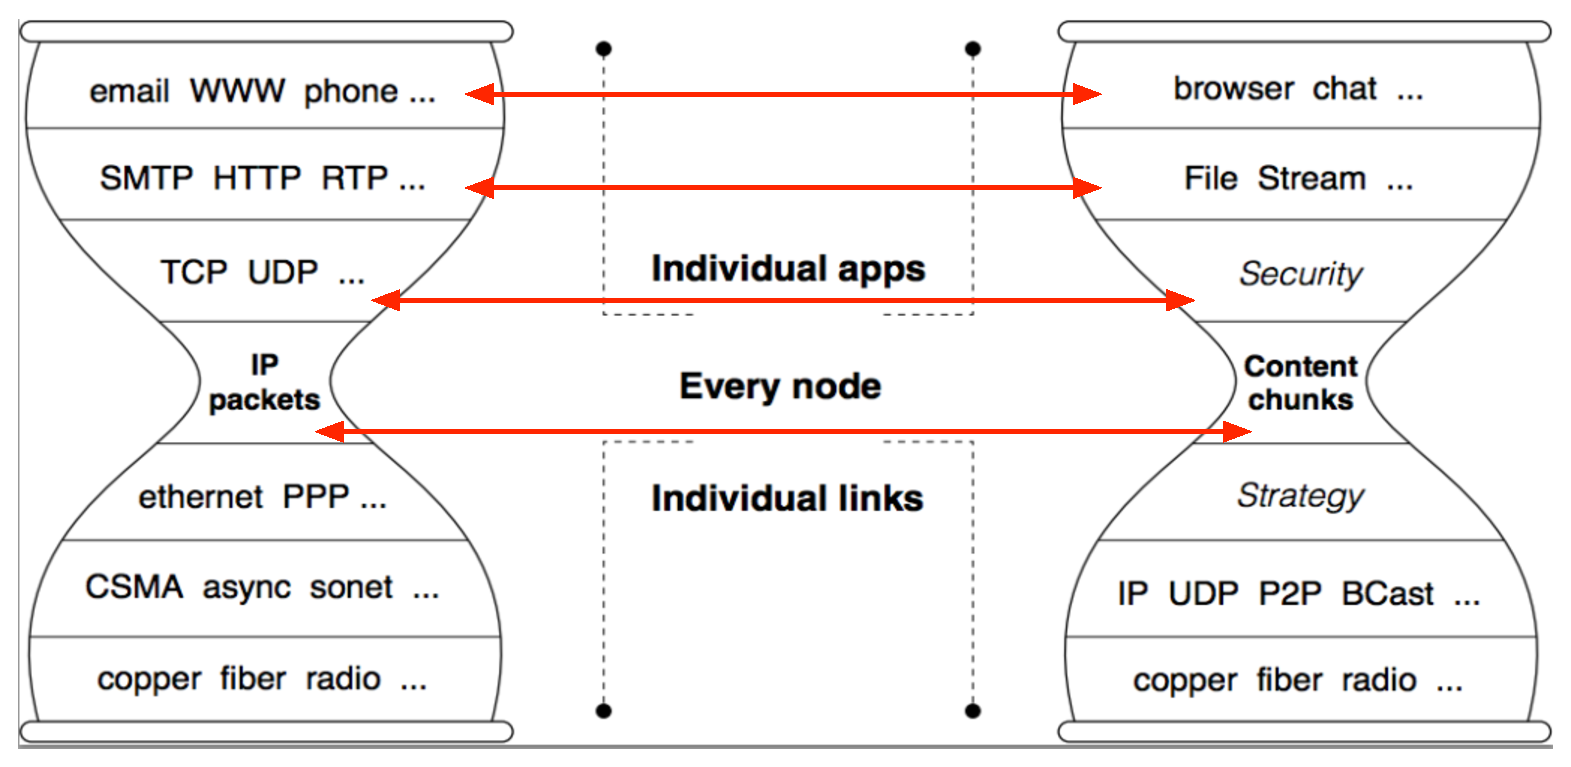
\includegraphics[scale=0.32]{./images/hourglass_conn.pdf}
\label{fig:hourglass}
\caption{A visual comparison of the network stacks for the IP and NDN network architectures (figure from \cite{ndn-techreport}).}
\end{center}
\end{figure}

Assuming that NDN is not to be deployed over IP, but instead as a separate network stack entirely, the need for such a gateway cannot be understated. Consider two instances of an application, $A$ and $B$, that wish to send data back and forth to each other. Application $A$ is running on a host with only an IP interface, and application $B$ is running on a host with only an NDN interface. What does it mean for application $A$ to establish a TCP connection stream with application $B$ and what does it mean for application $B$ to issue an interest to application $A$ when neither application speaks the network language of the other. In order for these two applications to communicate, the semantics of a TCP stream-oriented connection must be translated to a stream of contiguous interests, and vice versa. Now consider the alternative scenario in which two or more physically disjoint NDN networks need to communicate to distribute content, but such networks can only be connected via the Internet. Strategically placed border gateways at the edges of these NDN networks can be used to establish a bridge across the Internet to enable cross-network interest issuance and content retrieval. Given these two seemingly unavoidable scenarios in an incremental deployment of NDN networks, our IP/NDN bridge will enable continual application operation with minimal application and transport layer software changes. In the following sections we describe the gateway design that faciliates such interoperability.

% The gateway middleware is designed so as to support bi-directional traffic flowing from both types of networks. In what follows we describe how traffic in both directions will be supported internally by the gateway.

% \begin{table}[t]
%     \begin{tabular}{|c||c|c|}
%     \hline
%     ~    & {\bf IP} & {\bf NDN} \\ \hline
%     {\bf HTTP} & ~ & ~ \\ \hline
%     {\bf FTP}  & ~ & ~ \\ \hline
%     {\bf SMTP} & ~ & ~ \\ \hline
%     {\bf DNS}  & ~ & ~ \\ \hline
%     \end{tabular}
% \end{table}

% \todo[inline]{gateway is two-sided facade}

\section{Network Semantic Translations at the Gateway} \label{sec:gateway}
Traditional IP-based applications and upcoming NDN-based applications treat both the network and content in significantly different ways. In IP-based settings, application and transport layer mechanisms and protocols leverage the underlying IP network layer to send packets to specific hosts. In contrast, in NDN-based settings, there are no straightforward application or transport layer analogs; the network layer, responsible for the issuance of interests and retrieval of content, is abstracted to authenticated (i.e., digitally signed) content objects or streams of data that are consumed by applications. From this perspective, there is no clear bijection between application and transport layer communication in IP-based settings and content and stream-centric data retrieval in NDN-settings. Therefore, to support the interoperability of these two networking paradigms, we need a mechanism to translate the semantics of IP-based communication to and from NDN-based content retrieval. 

The direction of traffic across the gateway has a strong influence on how this semantic translation is done: IP-to-NDN application and transport layer protocols will be mapped to corresponding NDN-interests, and NDN-to-IP traffic (in the form of interests) will be encoded so as to map to the appropriate IP-based application or transport layer protocol. Stateless protocols such as HTTP greatly simplify the job of the gateway because it need not maintain any state to support communication across both networks. However, stateful protocols, such as TCP, naturally require the gateway to maintain state so as to emulate the behavior of an endpoint or host that implements such protocols. For instance, if an IP-based application wishes to establish a TCP connection with an application running on an NDN network to retrieve data, then the gateway must maintain stateful information needed to transform streams of data retrieved over a TCP socket to (packed) discrete and contiguous interests in the NDN network. In what follows we describe the semantic translation details for application and transport layer stateful and stateless protocols in both directions across the gateway. 

\subsection{IP-to-NDN Semantic Translation}
The current CCNx libraries enable IP-based hosts to communicate with applications running on NDN-enabled hosts. However, the engineering effort to retrofit the entire networking layer or subsystem of an existing applications or systems could be quite significant. The gateway is designed to minimize the effect of modifying the network components of such applications to still communicate with NDN hosts. In particular, it enables existing IP-based protocols to be used as is or with slight variations (e.g., TCP connections require additional overhead to setup) to communicate with NDN hosts through the gateway. In this way, the semantic translation of IP-based messages to NDN-based interests and content is offloaded to the gateway, rather than done in the application itself. In the following sections we describe the steps necessary to interoperate with the gateway at both the application and transport layers, which are the two most common levels used by applications for point-to-point communication in the OSI network stack.

% TODO: could link in CCNx library and re-write networking code, but that requires too much work, instead we re-use existing protocols for encoding interests

\subsubsection{Application Layer}
Translating IP-based application layer messages to NDN interests is highly dependent on the particular application protocol in question. There is an intuitive NDN-friendly encoding of HTTP GET requests in which human-readable URIs are parsed as interest names. Stateless application-layer protocols enable such direct mappings. Therefore, the gateway supports IP-to-NDN application layer messaging by encoding interests in HTTP GET requests as follows. NDN content objects with names ``ccnx:/name/of/content'' are issued via the gateway by sending a HTTP GET request with the following format to the gateway (in this example, the IP address X.X.X.X of the gateway is known or can be obtained via DNS):
\begin{center}
{\tt GET X.X.X.X:80/ndn/ccnx/name/of/content}
\end{center}
Since HTTP requests and NDN interests are stateless, the gateway will parse the URI of the request to determine that (1) it corresponds to an NDN interest, and (2) the full interest name is explicitly ``ccnx:/name/of/content''. Upon reception, the gateway will store the key-value pair $(\mathsf{name}, (\mathsf{source-IP}, \mathsf{source-port}))$ in the IP pending message table and issue an interest with the given name to the NDN network. Upon receipt of a piece of content, a NDN content handler callback recovers the IP address and port from the pending message table using the content name as the index and then writes the raw content back to the client over the same incoming HTTP TCP connection. Since it is not required that the HTTP request uses a persistent TCP connection, the HTTP message handler is a synchronous procedure that blocks while the NDN interest is satisfied so that the same TCP connection can be used to write the response. 

\subsubsection{Transport Layer} % ip to ndn
Since interests can be overloaded to contain arbitrary data, our gateway design exploits this characteristic to carry transport-layer streams of data from applications on IP hosts to supporting applications on NDN-hosts. IP is a host-based protocol, however, and so establishing a ``virtual'' TCP connection between two such applications must be done in two steps: (1) a TCP socket from the IP client to the gateway must be established, and (2) the first chunk of data sent from the client must be the NDN host prefix to which data will be sent. The gateway parses this path and stores it internally for each open TCP socket. Let $C$ be the IP client generating data in the socket $\mathsf{socket}$ from source address and port $(A, P)$, let $(pk,sk)$ be a public and private key pair owned by $C$, and let $G$ be the gateway forwarding data on behalf of $C$. The connection establishment phase proceeds as follows:
%
\begin{compactenum}
	\item $C$ opens a TCP socket connection $\mathsf{socket}$ to $G$. \item Let $\mathsf{id}$ be a unique identifier for the TCP socket in both $C$ and $G$.
	\item $C$ sends $\mathsf{prefix}/\mathsf{EOC}$ to $G$ over $\mathsf{socket}$, where $\mathsf{EOC}$ is the end-of-connection indicator.
	\item $G$ reads and parses data from $\mathsf{socket}$, and stores the key-value pair $(\mathsf{id}, \mathsf{prefix})$ in the TCP connection map.
	% ??? need to send path and public key (we then compute the hash and save the TCP session identifier)
\end{compactenum}
%
With $\mathsf{prefix}$ and $\mathsf{id}$ generated during the the connection establishment phase, all subsequent data chunks are then forwarded to this NDN host using the following steps:
%
\begin{compactenum}
	\item $C$ sends a chunk of $b$ bytes to $G$ over the socket $\mathsf{socket}$.
	\item $G$ reads $b$ bytes of data from $b$ and encodes it in Base64 format, denoted as $\mathsf{data}$.
	\item $G$ generates a uniformly random string $\mathsf{nonce}$ of $k$ bits from $\{0,1\}^k$. 
	\item $G$ retrieves $\mathsf{prefix}$ from the TCP connection map using the TCP socket ID $\mathsf{id}$, uses it to build the interest $\mathsf{prefix}/\mathsf{nonce}/\mathsf{data}$, and issues the interest to the NDN network.
\end{compactenum}
%
By incorporating a fresh random string in each new interest name, the probability that any issued interest will be satisfied from a network cache instead of the desired NDN host is negligible. Therefore, all data sent over the socket $\mathsf{socket}$ will reach the NDN host, and the receiving application can parse the last component of the interest as fresh data. Note that since this is strictly IP-to-NDN communication, there is no state information persisted in the session table. This is because the NDN host application may not respond with data since the gateway is forwarding \emph{transport} layer data, unlike the case where application-layer queries are forwarded. If the target application wishes to respond, it may do so by retrieving the TCP session identifier from the interest name and responding with a properly formatted interest as specified below in Section \ref{sec:ndn-to-ip}.

% TODO: interests can be overloaded to contain content, some NDN applications will accept some interests, applications using raw TCP streams to send data to NDN applications, so client opens up TCP socket to gateway and all data is partitioned/packed in an interest/forwarded, setting up TCP connection requires hooking up socket to gateway/sending producer root as first message chunk in TCP stream/and then sending streams of data continually

\subsection{NDN-to-IP Layer Semantic Translation}\label{sec:ndn-to-ip}
Due to their architectural differences, there does not exist a native correspondence between NDN interests and IP-based application layer protocol messages. For example, there is no standard way for a client to represent an HTTP GET request in the format of an NDN interest. To make this type of semantic translation possible, the NDN-to-IP application layer bridge leverages the human-readable names of content to encode IP-based application layer protocol specifics. The grammar for encoding for HTTP and FTP semantic translations is specified in EBNF form in Figure 2; other application-layer protocols can easily be supported by extending this grammar in the natural way.

% \todo[inline]{Command pattern}

\begin{figure*}
\begin{mdframed}
\begingrammar
\noindent

<ip-interest>:	'/$\dots$/ip/'<protocol>.

<protocol>:	'http/'<http-cmd>[{'/'<http-path>}] | 'tcp/'<tcp-ident>'/'<uri-encoded-string>. 

<http-cmd>: 'GET' | 'PUT' | 'POST' | 'DELETE'.

% <ftp-cmd>: 'ascii' | 'binary' | 'bye' | 'cd' | 'close' | 'delete' | 'get' | 'help' | 'lcd' | 'ls' | 'mkdir' | 'mget' | 'open' | 'put' | 'pwd' | 'quit' | 'rmdir'.

<http-path>: <uri> | <ip-address>[port]['/'<uri-encoded-string>]

<tcp-ident>: <SHA256-hash>'/'<nonce>'/'<public-key>. % nonce is the random ID associated with the TCP socket for constant-time lookup when going from ndn-to-ip, this must be set during the connection establishment phase from ip-to-ndn (if it doesn't exist in the TCP state table, then the NDN-side is creating the connection in one shot)

<tcp-param>: <uri-encoded-string>.

% <number>:	<real-number>;
% 		"$\{$" <real-number> "," <real-number> "$\}$";
% 		{$\backslash$}b[01][01]+;
% 		{$\backslash$}o[07][07]+;
% 		\$[0-9A-Fa-f][0-9A-Fa-f]+.

%<real-number>:	[\+--]?[0-9][0-9]+[\.[0-9]+]?[[eE][0-9][0-9]+].

% <operator>:	"*" |	 "/"	|     "$\backslash$"	| "\%";
% 		"==" |	 "!="	|     "$>$" 		| "$<$"  
% 		| "$<$=" | "$>$=";
% 		"\ul ="	| "\ul !=" |  "\ul $<$" | "\ul $>$" 
% 		| "\ul$<$=" | "\ul$>$=";
% 		"\&"	 | "$\vert$"  | "$\uparrow\uparrow$";
% 		"\&\&"	| "$\Vert$"  | "\ul$\uparrow$".
		
\endgrammar
\end{mdframed}
\caption{NDN-to-IP application-layer translation encoding grammar.}
\end{figure*}

Interests encoded using this grammar are intercepted in the NDNInputStage of the gateway (see Figure \ref{fig:pipeline}). Upon reception, the gateway parses the message, stores a new entry in the NDN pending message table, and forwards the decoded message contents to the appropriate IPOutputStage pipeline stage. Upon reception, the IP response is retrieved in the IPInputStage and forwarded inwards to the NDNOutputStage, where the corresponding entry in the NDN pending message table is indexed using the contents of the arriving message to retrieve the original incoming interest name. Once fetched, the gateway creates and signs a new content object with the IP network response, and then forwards the content downstream to its intended consumer. 

Unlike traditional NDN routing, the gateway pending message table does not collapse interests by default. The reason for this is that application-protocol interests are often issued when \emph{new} state needs to change (i.e., cached responses not generated on demand from the intended IP recipient are not acceptable). 

It is important to note that stateful protocols such as TCP must explicitly embed identifying information about the consumer in order to operate correctly. The reason is that one TCP stream must be associated with at most one consumer, and since NDN does not have any notion of host addresses or identifiers, the consumer application must explicitly encode its identity in the interest. Our grammar enforces identities based on consumer public keys and a corresponding digital signature of the entire interest for such protocols so that consumers can be explicitly identified and their sessions cannot be hijacked by other consumers (doing so would require compromising a consumer and its private key).

\section{Bridging Isolated Networks} \label{sec:bridge}
The second type of interoperability scenario that may arise during the deployment of NDN networks is when two or more physically disjoint NDN networks need to communicate with eachother. Let $I_i$ and $I_j$ be two such dijoint NDN networks, and let $A_i$ and $A_j$ be two applications running on hosts in $I_i$ and $I_j$, respectively. Without any additional mechanisms, $A_i$ and $A_j$ would not be able to communicate. However, if there existed two bridges $B_i$ and $B_j$ at the edges of $I_i$ and $I_j$, each of which connected to the same IP-based network (i.e., the Internet), then interests from $A_i$ ($A_j$) could be sent to $A_j$ ($A_i)$ as follows:
\begin{compactenum} 
	\item An interest from $A_i$ is intercepted a bridge $B_i$.
	\item $B_i$ encapsulates the interest in an IP packet sent to brige $B_j$.
	\item $B_j$ unwraps and re-issues the interest and waits for the content to be retrieved from $A_j$. Upon reception, the content's signature is verified and the content is signed and sent to $G_i$. 
	\item $G_i$ verifies the signature of the packet, creates and signs a new content object, and sends the content object back downstream to $A_i$.
\end{compactenum}
A visual depiction of this scenario is shown in Figure \ref{fig:islands}. To increase interest throughput across the bridge, each bridge uses persistent content-oriented TCP connections between other adjacent bridges. In order to authenticate content sent between bridge, we have the option of establishing a secure connection via SSL/TLS so that all content messages will be authenticated below the application-layer of the bridge, or we can manually sign and verify content separately from transport mechanism. Since NDN/CCN stipulates that content is only signed (as a form of authentication), we do not need the additional overhead of encrypting content as it moves between bridges. This is why we provide support for secure and insecure persistent connections. 

\begin{figure}[ht!]
\begin{center}
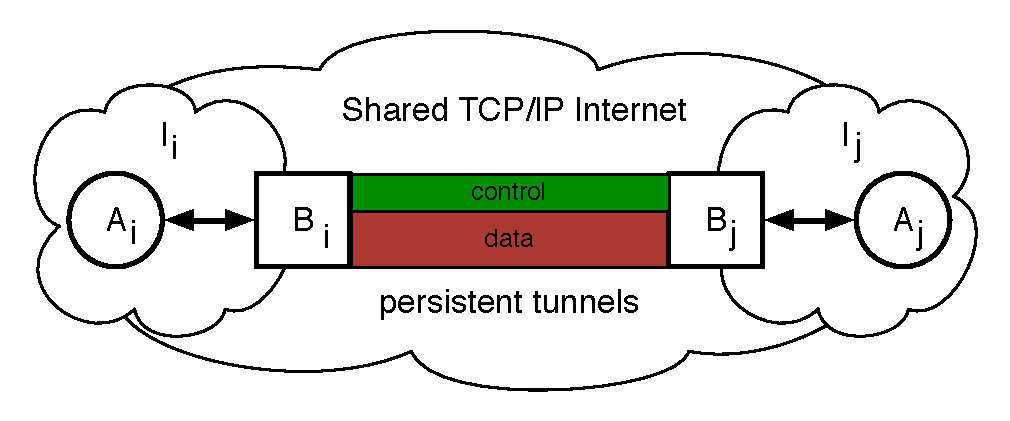
\includegraphics[scale=0.45]{./images/island_tunnel.pdf}
\label{fig:islands}
\caption{Visual depiction of a bridge between NDN islands.}
\end{center}
\end{figure}

In the latter case, one issue is the method for locating and retrieving cryptographic keys used for digital signatures. If the content TCP socket is not Our design permits three variations for authenticating content between bridges: (1) full PKI-based based digital signatures, (2) keyed MAC tags sourced by keys generated from authenticated symmetric key agreement protocols (i.e., Diffie Hellman key agreement), and (3) keyed MAC tags sourced by a \emph{shared} symmetric key bridge group key generated using a group key agreement protocol (i.e., Tree-Based Group Diffie Hellman). In what follows we describe each of these three variants in more detail; modifications to the content authentication procedure described above between bridges change in the obvious way (i.e., keyed MAC tags are replace digital signatures for MAC-based variants) Figure \ref{fig:gateway-groups} shows a visual depiction of the variants (1) and (2). \\

\begin{description}

	\item[\textbf{Full PKI-based Digital Signatures}:] The only modification required for this variant is that bridges must be given the certificate for each bridge with which it will communicate. Certificates are exchanged and stored via the control channel between adjacent bridges.

	\item[\textbf{Pair-Wise Keyed MAC Tags}:] In this variant, each pair of bridges will run the DH protocol to establish a shared common symmetric key to use for generating MAC tags. The DH protocol is run over the control channel between adjacent bridges. With $n$ bridge routers, this variant requires $frac{n(n-1)}{2}$ key pairs. MAC keys need to only be refreshed when they expire out or the bridge connectivity changes. New bridges can discover all other bridges by querying a central ``gateway directory'' server, obtaining a list of all corresponding IP addresses, and then initiating control channel connections with them.

	\item[\textbf{Group-Based Keyed MAC Tags}:] When all groups share a common key, the ``bridge directory'' server is repurposed as a distributed director for all registered bridges that is responsible for coordinating group key agreement protocols (i.e., TGDH \cite{kim2004tree}). After a single invocation of TGDH, each gateway will possess the same MAC key $k$ used for tagging and verifying content. Each individual bridge is also required to periodically send heartbeat messages to the director in order to maintain an active list of available bridges. The director will initiate new instances of the TGDH protocol to establish a new shared group key whenever bridge connectivity changes, i.e., when new bridges are added or time out. 

\end{description}

\begin{figure}[ht!]
\begin{center}
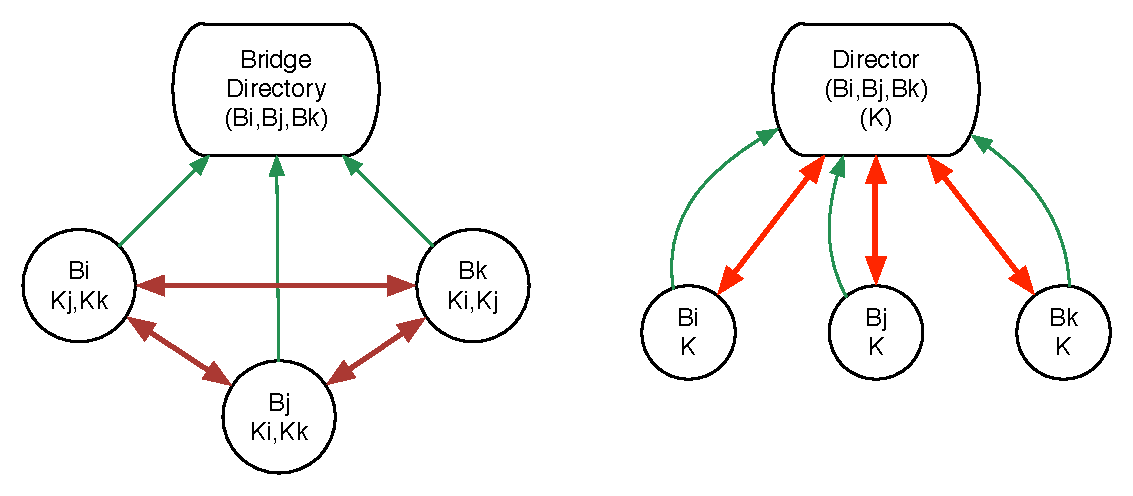
\includegraphics[scale=0.45]{./images/gateway_group.pdf}
\label{fig:gateway-groups}
\caption{The left figure shows the deployment strategy with a fixed global directory that exists merely for obtaining bridge addresses, and the right figure shows the deployment strategy in which a distributed directory coordinates group key agreement protocols between all bridges.}
\end{center}
\end{figure}

Another issue is that incoming interests need to be directed to bridges connected to the desired endpoint network. We achieve this by maintaining a prefix-bridge mapping $\mathsf{PTGMap}$ in each bridge $B_i$ about interest prefixes and the associated bridges from which they can be satisfied. If an incoming interest to bridge $B_i$ has no key in $\mathsf{PTGMap}$, i.e., a previous interest with the prefix $\mathsf{p}$ was never received by $B_i$, then the interest is broadcast to all known bridges. Whenever a response is retrieved from a source bridge $B_j$, the key-value pair $(\mathsf{p}, G_j)$ is inserted into $\mathsf{PTGMap}$. All subsequent interests with the prefix $\mathsf{p}$ received by bridge $B_i$ will be sent directly to bridge $B_j$. If an interest times out, the $\mathsf{PTGMap}$ entry is removed, and the broadcast procedure is retried. 

% \begin{algorithm}[ht!]
%   \caption{EstablishBridge}
%   \begin{algorithmic}[1]
%     \Require{Anonymous routers $r_1,r_2,\dots,r_n$ ($n \geq 1$) with public keys $pk_1,pk_2,\dots,pk_n$.}
    
% % \medskip

% % \Function{{\sf InitHandler}}{$\mathsf{int}$} %// Server-side at router $i$
% %     \State $(k, E_{k_i}, M_{k_i}, M_{k_{i+1}}, \mathsf{EIV}_i, \mathsf{SIV}_i^1, \mathsf{session}_i, \mathsf{SIndex}_i^1) := \mathcal{D}_{sk_i}(\mathsf{int})$
% %   \State Persist $(\mathsf{session}_i, E_{k_i}, M_{k_i}, M_{k_{i+1}}, \mathsf{EIV}_i, \mathsf{SIV}_i)$ to state, and store $(\mathsf{SIndex}_i, \mathsf{session}_i, \mathsf{SIV}_i)$ in the session table $\mathsf{ST}_i$
% %   \State $\mathsf{resp} \gets \mathsf{Encrypt}_{k}(\mathsf{session}_i, E_{k_i}, M_{k_i}, \mathsf{EIV}_i, \mathsf{SIV}_i)$
% %   \State \Return $\mathsf{resp}$
% %  \EndFunction

% % \medskip

% % \Function{{\sf Init}}{$r_i$, $M_{k_{i+1}}$} %// Client-side
% %   \State $E_{k_i} \gets \{0,1\}^{\kappa}, M_{k_i} \gets \{0,1\}^{\kappa}$
% %   \State $\mathsf{EIV}_i \gets \{0,1\}^{\kappa}, \mathsf{SIV}_i^1 \gets \{0,1\}^{\kappa}$ %// session IV
% %   \State $x \gets \{0,1\}^{\kappa}, \mathsf{session}_i := H(x)$ %// session ID
% %   \State $\mathsf{SIndex}_i^1 := H(\mathsf{session}_i + \mathsf{SIV}_i)$
% %   \State $\mathsf{PAYLOAD} := \mathcal{E}_{pk_i}(k, E_{k_i}, M_{k_i}, M_{k_{i+1}}, \mathsf{EIV}_i, \mathsf{SIV}_i, \mathsf{session}_i, \mathsf{SIndex}_i^1)$
% %   \State $\mathsf{int} := \mathsf{namespace}_i/\mathsf{CREATEInitHandlerSION}/\mathsf{PAYLOAD}$
% %   \State $\mathsf{resp} := \mathsf{ccnget}(\mathsf{int})$ %// reach out to the AR
% %   \State \Return $(E_{k_i}, M_{k_i}, x_i, \mathsf{session}_i, \mathsf{IV}_i)$
% % \EndFunction

% % \medskip

% % \Function{{\sf EstablishCircuit}}{$r_1,\dots,r_n$} %// Main procedure
% % \State $(E_{k_n}, M_{k_n}, c_n, \mathsf{session}_n, \mathsf{IV}_n) := \mathsf{Init}(r_n)$
% % \For{$i = n - 1$ \textbf{ downto } $1$}
% %   \If{$i = n-1$}
% %     \State $(E_{k_i}, M_{k_i}, \mathsf{EIV}_i, \mathsf{session}_i, \mathsf{SIV}_i) := \mathsf{Init}(r_i, \perp)$
% %   \Else
% %     \State $(E_{k_i}, M_{k_i}, \mathsf{EIV}_i, \mathsf{session}_i, \mathsf{SIV}_i) := \mathsf{Init}(r_i, M_{k_{i+1}})$
% %   \EndIf
% % \EndFor
% % \EndFunction

%   \end{algorithmic}
%   \label{alg:init}
% \end{algorithm}
\section{Implementation Overview}
\sink\ is implemented entirely in Python using the PyCCN \cite{pyccn} wrapper around CCNx. Currently, all functionality except transport layer semantic translation is implemented. The design of \sink\ can be viewed from two perspective: the gateway component and the bridge component. Though the bridge component uses elements of the gateway to minimize redundant code, the designs of each are mostly independent. In this section we describe each of them in more detail. 

\subsection{Gateway Implementation}
The core design of the gateway can be perceived as the composition of two flexible pipelines that route traffic from NDN (resp. IP) networks to IP (resp. NDN) networks (see Figure \ref{fig:pipeline}). Each pipeline begins and ends with an {\tt InputStage} and {\tt OutputStage}, respectively, one for the IP network and one for the NDN network. Each {\tt InputStage} instance runs an appropriate interface to the network from which it receives traffic. Specifically, the {\tt IPInputStage} runs an HTTP server to intercept IP-to-NDN interests, and the {\tt NDNInputStage} registers a CCNx handle and configures an interest filter for incoming interests. 

\begin{figure*}[ht!]
\begin{center}
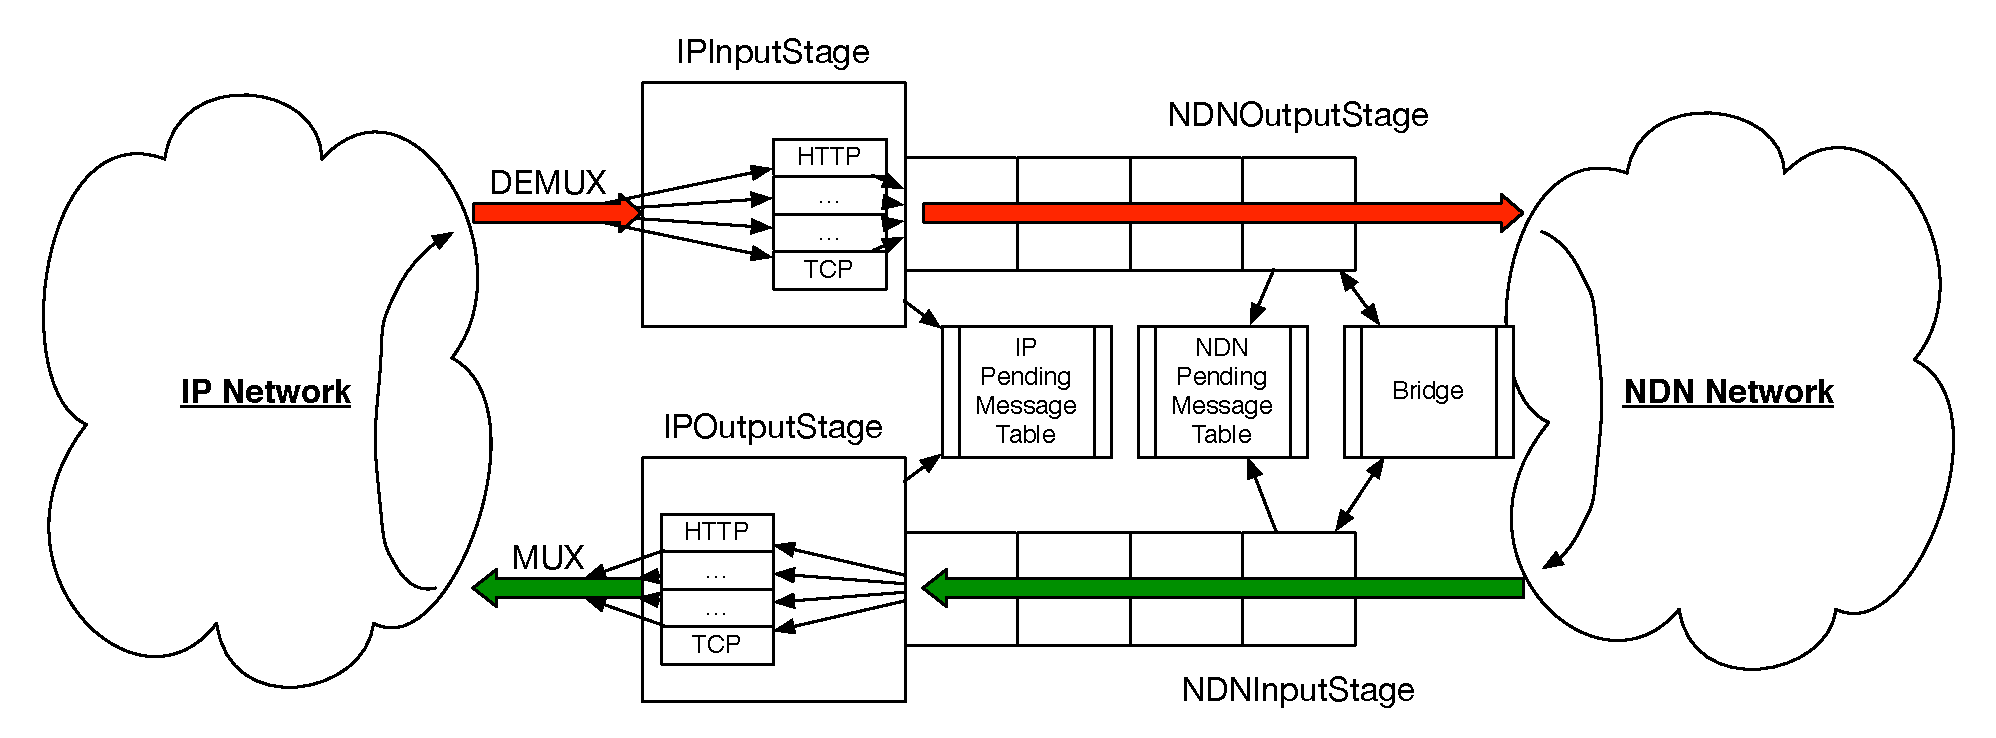
\includegraphics[scale=0.45]{./images/pipeline.pdf}
\label{fig:pipeline}
\caption{Bidirectional message pipeline for IP-to-NDN and NDN-to-IP message traversal.}
\end{center}
\end{figure*}

It is important to emphasize that the {\tt NDNInputStage} operates independently of the underlying network implementation. In a true deployment, CCNx would not be used to interface with the NDN network. Rather, a CCN network stack would be implemented on top of the appropriate network interface controller (NIC). The mechanism for registering an interest filter on top of this network stack would change, but the functionality that happens after an interest is intercepted will remain the same. Using CCnx for the preliminary development of this gateway was necessary since there does not yet exist NDN NICs or CCN software stacks that are not built upon the TCP/IP stack.

After an input stage receives an incoming message (i.e., an IP packet or NDN interest), the asynchronous message handler will (1) allocate an entry in the \emph{pending message table} for the network interface, (2) decompose the components of the message into its ``raw form'' and (3) save them in common message object wrapper, and (4) forward the resulting object to the next pipeline stage. For example, the {\tt IPInputStage} will save the IP source host and port information in the {\tt IPPendingMessageTable}, extract the URI path and set it as the ``destination'' field in the outgoing message object, and forward this message object to the next pipeline stage. In addition to the message source information for each entry in the pending message table, a binary semaphore is also stored. After forwarding the object, each handler will acquire a lock on this binary semaphore until the content associated with this message is retrieved from the target network. 

The pipeline is designed so that each stage (with the exception of the {\tt InputStage}) has a thread-safe input queue and a reference to the next stage (with the exception of the {\tt OutputStage}). This simple interface and design enables any number of intermediate stages to be configured between the input and output stages. For simplicity, the current \sink\ implementation only uses two stages - input and output stages. 

Once a message reaches the output stage, a new message for the target network is created and issued to the network. For example, an NDN interest will be formatted based on the contents of the outgoing message object retrieved from the output stage queue. After the target network returns content, the input stage of the target network performs the following tasks: First, the pending message table is checked for the an entry corresponding to the input message (e.g., an interest name that matches name of a previously issued interest). If an entry is found, the content field of the matching entry is populated and the binary semaphore associated with the semaphore is released. The latter step unblocks the original asynchronous input stage message handler, which then retrieves the content from the pending message table entry and sends it to the original consumer. If a matching entry in the pending message table is not found, the incoming message is treated as a ``new'' message, and it is formatted and flows through the pipeline in the opposite direction. 

% \todo[inline]{pipeline stage defers parsing to subclasses - template pattern}

\subsection{Bridge Implementation}
As illustrated by Figure \ref{fig:pipeline}, the bridge component of \sink\ is designed to interoperate with the input and output stages of the gateway. The current implementation uses a central directory to manage bridge locations and status updates (see Section \ref{sec:bridge}). Additionally, due to the small scale at which \sink\ was tested, the pair-wise MAC key management scheme is implemented. The design and implementation does not impede the integration of the more efficient TGDH protocol that is also discussed in Section \ref{sec:bridge}. Each instance of \sink\ runs a separate thread for the bridge component that manages the following tasks:
\begin{compactitem}
	\item Sending periodic heartbeat messages to the bridge.
	\item Establishing and storing pair-wise MAC keys with all known bridges.
	\item Managing the {\sf PTGMap} table.
	\item Controlling selective interest forwarding to specific bridges or broadcasting to all known bridges.
\end{compactitem}

The bridge component in $B_i$ leverages the {\tt NDNInputStage} and {\tt NDNOutputStage} in the following way: If the name of an arriving interest does not have the default gateway prefix as specified in Section \ref{sec:gateway}, the interest is forwarded to the queue of the bridge thread. This bridge thread then extracts the interest from the queue and checks the {\sf PTGMap} map for the interest prefix. If a match is found for prefix $\mathsf{prefix}$, the interest name is sent to the mapped bridge $B_j = \mathsf{PTGMap}[\mathsf{prefix}]$ over a persistent TCP stream. If a prefix match is not found in the {\sf PTGMap}, then the interest name is broadcasted to all bridges over their respective TCP streams. After sending this interest, $B_i$ will spawn a new thread that blocks until receipt of a response $r = (c,t)$ from the target bridge $B_j$. 

Upon receiving an interest at the target bridge $B_j$, an entry ($\mathsf{name}, \mathsf{socket}$) (where {\sf name} and {\sf sock} are the interest name and socket connection from which the interest was received) is created. The bridge then inserts this entry in a separate pending interest table so that the content response can be streamed back to the appropriate socket when retrieved. Then, an {\tt OutgoingMessage} with the interest is created and inserted into the local {\tt NDNOutputStage} queue. When content is eventually returned, the {\tt NDNInputStage} will examine the bridge pending interest table for the interest name to retrieve the socket object that will be used to send the response $r = (c,t)$, where $c$ is the content and $t$ is $\mathsf{HMAC}(K_i, c)$ (i.e., the keyed MAC tag generated with key $K_i$ associated with the recipient bridge $B_i$).

When $B_i$ receives a response $c = (c,t)$ from a socket connected to $B_j$, the MAC tag is verified. If the tag is valid, the content $c$ is returned to the original consumer and the content name prefixes are inserted into the {\sf PTGMap} table along with the address of $B_j$. If the tag is invalid, the content is ignored and the {\sf PTGMap} table is not updated. 

\subsection{Implementation Difficulties}
There were several implementation difficulties encountered during the course of this project. For brevity, we enumerate them below.
\begin{compactenum}
	\item Since TCP streams were used to transmit key data, interests, and content between bridges, we needed a simple way to encode and isolate each of these respective messages in the stream. To accomplish this task, we prepend each type of message with a single byte identifying the type of message to be sent (e.g., key data messages are prepended with the byte ``k'') and end each message with a {\tt \\n} character. The newline character is escaped in all content messages so as to avoid premature escapes and corrupt TCP streams.
	TCP message formatting
	\item Interfacing with the bridge directory needed to be a simple task that should be handled independently of the programming language used to implement the bridge clients. Therefore, we encode update messages in HTTP POST messages that can be formulated from any bridge client. The Python Flask web server enables us to easily parse and handle these HTTP messages, and the use of an application-layer protocol to send these messages allows us to re-implement the bridge client in any programming language should the need arive. For example, if we need to implement the bridge in C/C++ for increased performance, the bridge directory HTTP API does not permit us from doing so.
	\item Since we use the HMAC algorithm to tag and verify content sent between adjacent bridges, we needed to implement or find existing code for generating keys and computing this function. In the end, we settled on a hybrid approach in which the keys are generated using custom-written Diffie Hellman procedures and the HMAC function is computed using the Python {\tt hmac} library. Separating key establishment from the HMAC computation gave us added flexibility in how key shares are generated by the bridge components (i.e., we could generate key shares on demand in TCP servers in response to key messages from a TCP client). Additionally, using the existing HMAC implementation reduced the likelihood of bugs in the critical cryptographic code.
\end{compactenum}
\section{Performance Evaluation}
To evaluate the performance of \sink, we are concerned with (1) the overhead incurred by the semantic translation methods discussed in Section 4, (2) the message latency when crossing between different networks (e.g., the RTT of IP-to-NDN messages), and (3) the latency of messages traversing NDN bridges. Since key generation and directory updates happen infrequently and asynchronously, we did not measure the time to perform these tasks; we leave such evaluation to future work. To assess each of these measurements, we deployed a single bridge directory server that managed four (geographically) remote clients. Each of these hosts were running Ubuntu 12.10 and ran CCNx 0.8.1 and Python 3.1. Cryptographic libraries such as OpenSSL were not used for MAC tag generation and verification. 

Measurements (1) and (2) were tested via scripts that issue a series of IP-to-NDN and NDN-to-IP requests and record the time to retrieve a response. The overhead of translating IP to NDN messages was approximately 0.00078s for interest names composed of one (1) to five (5) components. Similarly, the overhead of translating NDN to IP messages was slightly higher with an average time of 0.0005s. Clearly, this overhead is negligible for sequential requests generated by small loads. Due to a lack of resources, large-scale tests were not conducted to see how this overhead increased with request load. Measurement (3) was tested by two remote clients connected to the central bridge directory. A script running on one client issued a series of NDN interests (via {\tt ccnpeek}) on one client (to be forwarded to the other client and satisfied by its set of connected hosts), and the RTT to retrieve content for each invocation of {\tt ccnpeek} was recorded. 

The RTT results for measurements (2) and (3) when retrieving content of roughly 1MB and 10MB in size is shown in Figures \ref{fig:perf1} and \ref{fig:perf2}. Our results indicate that IP-to-NDN and bridge message latencies were fairly consistent, whereas NDN-to-IP content retrieval incurred sporadic spikes in RTT. We attribute these anomalies to Python's thread synchronization primitives. 

\begin{figure}
\begin{center}
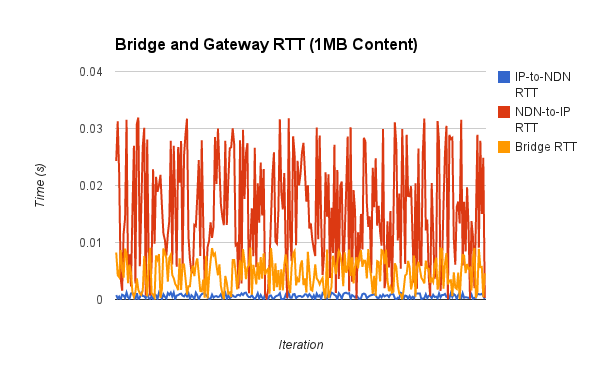
\includegraphics[scale=0.4]{./images/small.png}
\label{fig:perf1}
\caption{Average RTT times for IP-to-NDN, NDN-to-IP, and bridge messages when requesting content of approximately 1MB in size.}
\end{center}
\end{figure}

\begin{figure}
\begin{center}
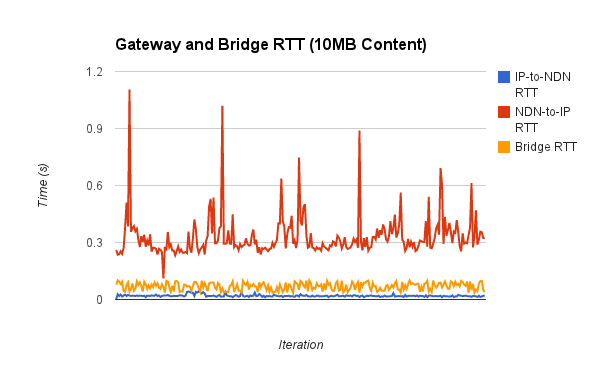
\includegraphics[scale=0.4]{./images/large.png}
\label{fig:perf2}
\caption{Average RTT times for IP-to-NDN, NDN-to-IP, and bridge messages when requesting content of 10MB in size.}
\end{center}
\end{figure}

% - test machine setup
% - experimental procedures and applications
% - link to source code
% - message translation overhead both ways
% - unidirectional and bidirectional RTT
% - bridge latency
% - say key generation and directory updates are asynchronous and one-time (don't happen a lot, so we didn't measure them)


\section{Related Work}
Little work has been done to evolve existing TCP/IP applications to correctly operate in the presence of NDN resources. NDNPurple is the only published work dealing with this issue \cite{wang2010implementing}. This NDN-based middleware is designed to allow existing TCP/IP instant messaging applications based on the XMPP protocol, which is implemented on top of the libpurple library, to operate over an NDN network. To accomplish this task, NDNPurple re-implemented the networking layer of the libpurple library to interface with an NDN proxy that communicates with other proxies for other parties in a single ``chat room.'' The proxy is responsible for marshalling buddy-list update requests and overloaded message content interests to all communication proxies. Additionally, the proxy is responsible for intercepting XMPP control messages (e.g., session keep-alive message) issued from the libpurple library and responding with the appropriate response. This proxy-based design enables chatrooms to be created in an ad-hoc manner, i.e., without a centralized server that manages chatroom session information. 

Beyond this simple proof-of-concept IP-to-NDN application evolution, there has been no other published work dealing with IP/NDN interoperability (in the same spirit of this work). 





\section{Conclusion}
We presented \sink\ , a middleware application that enables TCP/IP and NDN/CCN network interoperability. \sink\ is expected to aid incremental deployment of pure NDN/CCN networking resources by allowing applications implemented on top of different networking stacks to communicate with each other almost transparently using existing protocols via the middleware; for example, the use of overlay network libraries such as CCNx does not need to be implemented in each TCP/IP application that wishes to communicate with applications running on NDN/CCN hosts. Furthermore, the design and implementation of \sink\ is simple and flexible enough to permit more meaningful semantic translations between different network protocols while introducing minimal performance overhead in message latency. 

While the design is still rudimentary, there are several opportunities for improvement. From a design perspective, for example, the NDN-to-IP translation encoding grammar can be expanded to support additional TCP/IP application layer protocols, such as FTP, DNS, etc. The difficulty in encoding these types of application-layer protocols is that some of them require stored state and private client identification information. For example, if an anonymous FTP server is to be accessed via an NDN-based application, the \sink\ gateway must maintain a persistent FTP connection to the target server so that all issued commands can be executed. For example, the gateway must (1) establish a connection to the FTP server, (2) associate the connection with a \emph{single} NDN consumer, which can be identified via a hash of their public key, and (3) use this connection whenever the NDN consumer issues new commands (e.g., ``cd'' commands). The current design does not include a storage for such application-layer protocol state, but this could easily be fixed by including a helper state management class that is referenced by the appropriate pipeline stage. 

From an implementation perspective, the the bridge directory can be implemented as a set of distributed servers for increased performance under a large number of bridge clients generating heavy loads. Since we did not have access to a large set of clients to stress test the bridge directory, we are not sure how well the current implementation will scale. Such tests will also help us identify an appropriate frequency at which ``heartbeat'' messages are sent to the bridge directory. That is, if the design does not scale well under heavy loads, we can reduce the rate at which heartbeat update messages are sent to avoid self-induced denial-of-service attacks. Furthermore, pair-wise bridge keys can be replaced with shared group keys instantiated via group-key agreement protocols such as to TGDH. We are unaware of any open implementations of these cryptographic primitives, so we would need to construct them using the Python cryptographic libraries. 

% \section{Acknowledgments}

\bibliographystyle{abbrv}
\bibliography{ref}  % sigproc.bib is the name of the Bibliography in this case


\end{document}


